\documentclass[tikz, border=5mm, 12pt]{standalone}
\usepackage{amsmath}
\usepackage{amsfonts}

\usetikzlibrary{arrows.meta,shadows,positioning,calc,decorations.markings}

\pgfdeclarelayer{timelines}
\pgfsetlayers{timelines,main}

\begin{document}

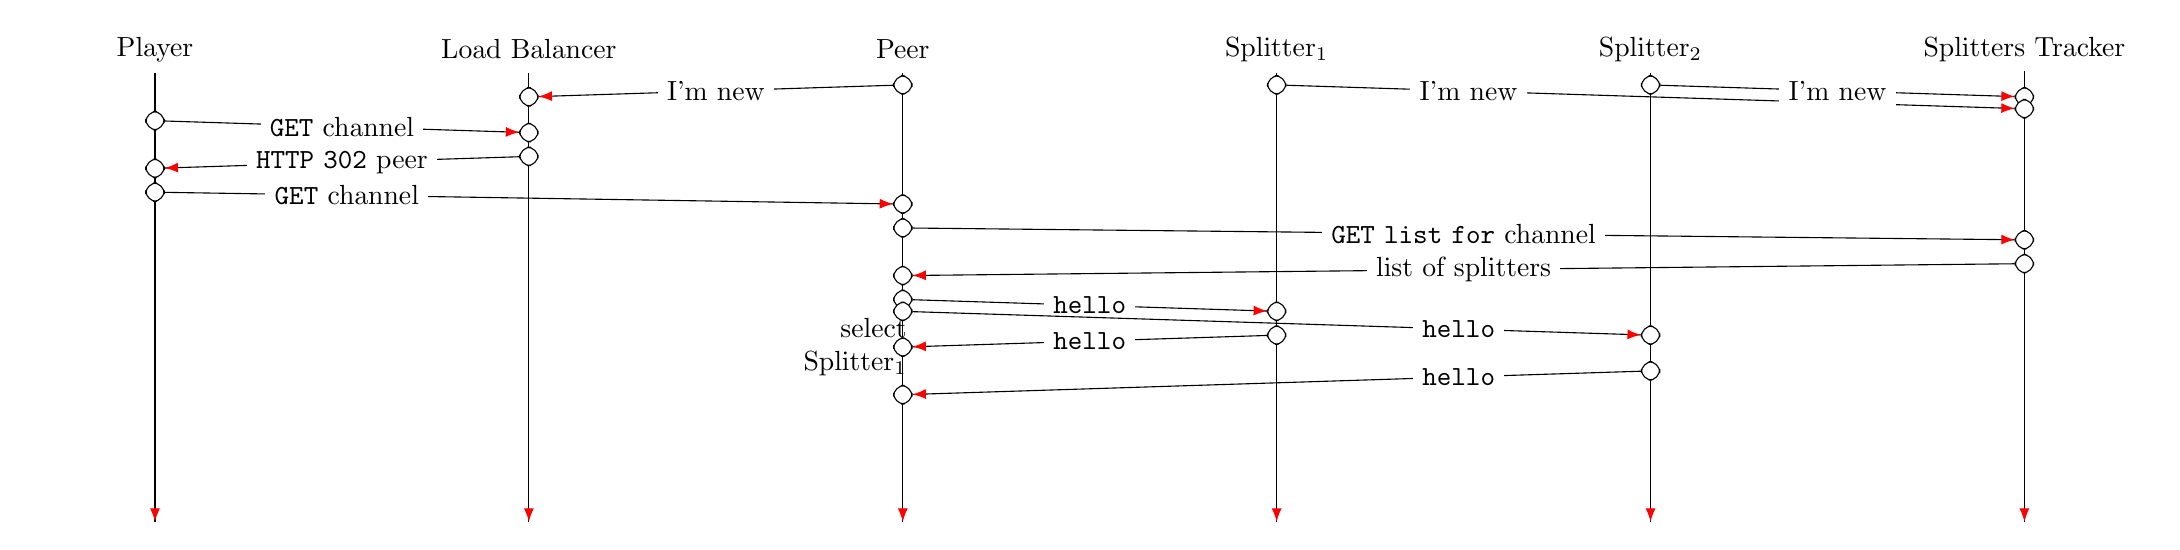
\begin{tikzpicture}
  
  \tikzset{myptr/.style={decoration={markings,mark=at position 1 with %
        {\arrow[red,scale=1.0,>=Latex]{>}}},postaction={decorate}}}
  
  % Entities
  \node[] (Player) {\parbox{3cm}{\centering Player}};
  \node[right=1.5 of Player] (Balancer) {\parbox{3cm}{\centering Load Balancer}};
  \node[right=1.5 of Balancer] (Peer) {\parbox{3cm}{\centering Peer}};
  \node[right=1.5 of Peer] (Splitter1) {\parbox{3cm}{\centering Splitter$_1$}};
  \node[right=1.5 of Splitter1] (Splitter2) {\parbox{3cm}{\centering Splitter$_2$}};
  \node[right=1.5 of Splitter2] (Tracker) {\parbox{3cm}{\centering Splitters Tracker}};

  % Timelines
  \begin{pgfonlayer}{timelines}
    \coordinate (Pla) at ($(Player.center) + (0.0,-6)$);
    \draw[myptr] ($(Player.center) + (0,-2ex)$) -- (Pla);  
    \coordinate (Bal) at ($(Balancer.center) + (0.0,-6)$);
    \draw[myptr] ($(Balancer.center) + (0,-2ex)$) -- (Bal);
    \coordinate (Pee) at ($(Peer.center) + (0.0,-6)$);
    \draw[myptr] ($(Peer.center) + (0,-2ex)$) -- (Pee);
    \coordinate (Sp1) at ($(Splitter1.center) + (0.0,-6)$);
    \draw[myptr] ($(Splitter1.center) + (0,-2ex)$) -- (Sp1);
    \coordinate (Sp2) at ($(Splitter2.center) + (0.0,-6)$);
    \draw[myptr] ($(Splitter2.center) + (0,-2ex)$) -- (Sp2);
    \coordinate (Tra) at ($(Tracker.center) + (0.0,-6)$);
    \draw[myptr] (Tracker) -- (Tra);
  \end{pgfonlayer}
  % Time steps
  
  % 00
  \node (00) at ($(Player) + (-2ex,-3ex)$) {};
  \node (Pe00) at ($(Peer) + (0,-3ex)$) [fill=white!100,draw,rounded corners] {};
  \node (Ba00) at ($(Balancer) + (0,-4ex)$) [fill=white!100,draw,rounded corners] {};
  \node (S100) at ($(Splitter1) + (0,-3ex)$) [fill=white!100,draw,rounded corners] {};
  \node (S200) at ($(Splitter2) + (0,-3ex)$) [fill=white!100,draw,rounded corners] {};
  \node (Tr001) at ($(Tracker) + (0,-4ex)$) [fill=white!100,draw,rounded corners] {};
  \node (Tr002) at ($(Tracker) + (0,-5ex)$) [fill=white!100,draw,rounded corners] {};
  \draw[myptr] (Pe00) -- (Ba00) node [pos=0.5,fill=white!100] {$\text{I'm new}$};
  \draw[myptr] (S100) -- (Tr002) node [pos=0.25,fill=white!100] {$\text{I'm new}$};
  \draw[myptr] (S200) -- (Tr001) node [pos=0.5,fill=white!100] {$\text{I'm new}$};
  
  % 01
  \node (01) at ($(00) + (0,-3ex)$) {};
  \path let \p{Player}=(Player),\p{01}=(01) in node (Pl01) at (\x{Player},\y{01}) [fill=white!100,draw,rounded corners] {};
  \node (011) at ($(00) + (0,-4ex)$) {};
  \path let \p{Balancer}=(Balancer),\p{011}=(011) in node (Ba01) at (\x{Balancer},\y{011}) [fill=white!100,draw,rounded corners] {};
  \draw[myptr] (Pl01) -- (Ba01) node [pos=0.5,fill=white!100] {$\mathtt{GET}~\text{channel}$};

  % 02
  \node (02) at ($(01) + (0,-3ex)$) {};
  \path let \p{Balancer}=(Balancer),\p{02}=(02) in node (Ba02) at (\x{Balancer},\y{02}) [fill=white!100,draw,rounded corners] {};
  \node (021) at ($(01) + (0,-4ex)$) {};
  \path let \p{Player}=(Player),\p{021}=(021) in node (Pl02) at (\x{Player},\y{021}) [fill=white!100,draw,rounded corners] {};
  \draw[myptr] (Ba02) -- (Pl02) node [pos=0.5,fill=white!100] {$\mathtt{HTTP~302}~\text{peer}$};

  % 03
  \node (03) at ($(02) + (0, -3ex)$) {};
  \path let \p{Player}=(Player),\p{03}=(03) in node (Pl03) at (\x{Player},\y{03}) [fill=white!100,draw,rounded corners] {};
  \node (031) at ($(02) + (0,-4ex)$) {};
  \path let \p{Peer}=(Peer),\p{031}=(031) in node (Pe03) at (\x{Peer},\y{031}) [fill=white!100,draw,rounded corners] {};
  \draw[myptr] (Pl03) -- (Pe03) node [pos=0.25,fill=white!100] {$\mathtt{GET}~\text{channel}$};

  % 04
  \node (04) at ($(03) + (0, -3ex)$) {};
  \path let \p{Peer}=(Peer),\p{04}=(04) in node (Pe04) at (\x{Peer},\y{04}) [fill=white!100,draw,rounded corners] {};
  \node (041) at ($(03) + (0,-4ex)$) {};
  \path let \p{Tracker}=(Tracker),\p{041}=(041) in node (Tr04) at (\x{Tracker},\y{041}) [fill=white!100,draw,rounded corners] {};
  \draw[myptr] (Pe04) -- (Tr04) node [pos=0.5,fill=white!100] {$\mathtt{GET~list~for}~\text{channel}$};

  % 05
  \node (05) at ($(04) + (0, -3ex)$) {};
  \path let \p{Tracker}=(Tracker),\p{05}=(05) in node (Tr05) at (\x{Tracker},\y{05}) [fill=white!100,draw,rounded corners] {};
  \node (051) at ($(04) + (0,-4ex)$) {};
  \path let \p{Peer}=(Peer),\p{051}=(051) in node (Pe05) at (\x{Peer},\y{051}) [fill=white!100,draw,rounded corners] {};
  \draw[myptr] (Tr05) -- (Pe05) node [pos=0.5,fill=white!100] {$\text{list~of~splitters}$};

  % 06
  \node (06) at ($(05) + (0, -3ex)$) {};
  \path let \p{Peer}=(Peer),\p{06}=(06) in node (Pe06) at (\x{Peer},\y{06}) [fill=white!100,draw,rounded corners] {};
  \node (061) at ($(05) + (0,-4ex)$) {};
  \path let \p{Peer}=(Peer),\p{061}=(061) in node (Pe061) at (\x{Peer},\y{061}) [fill=white!100,draw,rounded corners] {};
  \node (062) at ($(05) + (0,-6ex)$) {};
  \path let \p{Splitter1}=(Splitter1),\p{061}=(061) in node (S106) at (\x{Splitter1},\y{061}) [fill=white!100,draw,rounded corners] {};
  \draw[myptr] (Pe06) -- (S106) node [pos=0.5,fill=white!100] {$\mathtt{hello}$};
  \path let \p{Splitter2}=(Splitter2),\p{062}=(062) in node (S206) at (\x{Splitter2},\y{062}) [fill=white!100,draw,rounded corners] {};
  \draw[myptr] (Pe061) -- (S206) node [pos=0.75,fill=white!100] {$\mathtt{hello}$};

  % 07
  \node (07) at ($(06) + (0, -3ex)$) {};
  \path let \p{Splitter1}=(Splitter1),\p{07}=(07) in node (S107) at (\x{Splitter1},\y{07}) [fill=white!100,draw,rounded corners] {};
  \node (071) at ($(06) + (0,-4ex)$) {};
  \path let \p{Peer}=(Peer),\p{071}=(071) in node (Pe071) at (\x{Peer},\y{071}) [fill=white!100,draw,rounded corners] {};
  \node (072) at ($(06) + (0,-6ex)$) {};
  \node (073) at ($(06) + (0,-8ex)$) {};
  \path let \p{Peer}=(Peer),\p{073}=(073) in node (Pe073) at (\x{Peer},\y{073}) [fill=white!100,draw,rounded corners] {};
  \draw[myptr] (S107) -- (Pe071) node [pos=0.5,fill=white!100] {$\mathtt{hello}$};
  \path let \p{Splitter2}=(Splitter2),\p{072}=(072) in node (S207) at (\x{Splitter2},\y{072}) [fill=white!100,draw,rounded corners] {};
  \draw[myptr] (S207) -- (Pe073) node [pos=0.25,fill=white!100] {$\mathtt{hello}$};
  \node (Sel) at ($(Pe071) + (-4ex,0)$) {\begin{tabular}{r} select \\ Splitter$_1$ \end{tabular}};
  
\end{tikzpicture}
\end{document}

  % 04
  \node (04) at ($(03) + (0,-3ex)$) {04};
  \path let \p{04}=(04),\p{NAT A}=(NAT A) in node (N04) at (\x{NAT A},\y{04}) [fill=white!100,draw,rounded corners] {$\mathsf{A1}$};
  \path let \p{04}=(04),\p{Monitor}=(Monitor) in node (M04) at (\x{Monitor},\y{04}) [fill=white!100,draw,rounded corners] {$\mathsf{M}$};
  \draw[myptr] (N04) -- (M04) node [pos=0.5,fill=white!100] {$\mathtt{hello}~M$};

  % 05
  \node (05) at ($(04) + (0,-3ex)$) {05};
  \path let \p{Monitor}=(Monitor),\p{05}=(05) in node (M05) at (\x{Monitor},\y{05}) [fill=white!100,draw,rounded corners] {$\mathsf{M}$};
  \path let \p{NAT A}=(NAT A),\p{05}=(05) in node (N05) at (\x{NAT A},\y{05}) [fill=white!100,draw,rounded corners] {$\mathsf{A1}$};
  \draw[myptr] (M05) -- (N05) node [pos=0.5,fill=white!100] {$\mathtt{ack}~M$};

  % 06
  \node (06) at ($(05) + (0,-3ex)$) {06};
  \path let \p{NAT A}=(NAT A),\p{06}=(06) in node (NA06) at (\x{NAT A},\y{06}) [inner sep=0pt,minimum size=0pt] {};
  \path let \p{Peer A}=(Peer A),\p{06}=(06) in node (PA06) at (\x{Peer A},\y{06}) [inner sep=0pt,minimum size=0pt] {};
  \draw[myptr] (NA06) -- (PA06) node [pos=0.5,fill=white!100] {$\mathtt{ack}~M$};
  \path let \p{Splitter}=(Splitter),\p{06}=(06) in node (S06) at (\x{Splitter},\y{06}) [fill=white!100,draw,rounded corners] {$\mathsf{S}$};
  \path let \p{Monitor}=(Monitor),\p{06}=(06) in node (M06) at (\x{Monitor},\y{06}) [fill=white!100,draw,rounded corners] {$\mathsf{M}$};
  \draw[myptr] (M06) -- (S06) node [pos=0.5,fill=white!100] {$P_1=(\cal{A},\mathsf{A1})$};
  
  % 07
  \node (07) at ($(06) + (0,-3ex)$) {07};
  \path let \p{Monitor}=(Monitor),\p{07}=(07) in node (M07) at (\x{Monitor},\y{07}) [fill=white!100,draw,rounded corners] {$\mathsf{M}$};
  \path let \p{Splitter}=(Splitter),\p{07}=(07) in node (S07) at (\x{Splitter},\y{07}) [fill=white!100,draw,rounded corners] {$\mathsf{S}$};
  \draw[myptr] (S07) -- (M07) node [pos=0.5,fill=white!100] {$\mathtt{ack}~P_1$};

  % 08
  \node (08) at ($(07) + (0,-3ex)$) {08};
  \path let \p{Splitter}=(Splitter),\p{08}=(08) in node (S08) at (\x{Splitter},\y{08}) [fill=white!100,draw,rounded corners] {$\mathsf{S}$};
  \path let \p{NAT B}=(NAT B),\p{08}=(08) in node (NB08) at (\x{NAT B},\y{08}) [fill=white!100,draw,rounded corners] {$\mathsf{B0}$};
  \draw[myptr] (S08) -- (NB08) node [pos=0.5,fill=white!100] {$\{M,(({\cal{A}},{\mathsf{A0}}),\Delta_{\cal{A}})\}$};
  
  % 09
  \node (09) at ($(08) + (0,-3ex)$) {09};
  \path let \p{NAT B}=(NAT B),\p{09}=(09) in node (NB09) at (\x{NAT B},\y{09}) [inner sep=0pt,minimum size=0pt] {};
  \path let \p{Peer B}=(Peer B),\p{09}=(09) in node (PB09) at (\x{Peer B},\y{09}) [inner sep=0pt,minimum size=0pt] {};
  \draw[myptr] (NB09) -- (PB09) node [pos=0.5,fill=white!100] {$\{M,(({\cal{A}},{\mathsf{A0}}),\Delta_{\cal{A}})\}$};
  
  % 10
  \node (10) at ($(09) + (0,-3ex)$) {10};
  \path let \p{Peer B}=(Peer B),\p{10}=(10) in node (PB10) at (\x{Peer B},\y{10}) [inner sep=0pt,minimum size=0pt] {};
  \path let \p{NAT B}=(NAT B),\p{10}=(10) in node (NB10) at (\x{NAT B},\y{10}) [inner sep=0pt,minimum size=0pt] {};
  \draw[myptr] (PB10) -- (NB10) node [pos=0.5,fill=white!100] {$\mathtt{hello}~M$};
  
  % 11
  \node (11) at ($(10) + (0,-3ex)$) {11};
  \path let \p{NAT B}=(NAT B),\p{11}=(11) in node (NB11) at (\x{NAT B},\y{11}) [fill=white!100,draw,rounded corners] {$\mathsf{B1}$};
  \path let \p{Monitor}=(Monitor),\p{11}=(11) in node (M11) at (\x{Monitor},\y{11}) [fill=white!100,draw,rounded corners] {$\mathsf{M}$};
  \draw[myptr] (NB11) -- (M11) node [pos=0.25,fill=white!100] {$\mathtt{hello}~M$};
  \path let \p{Peer B}=(Peer B),\p{11}=(11) in node (PB11) at (\x{Peer B},\y{11}) [inner sep=0pt,minimum size=0pt] {};
  \draw[myptr] (PB11) -- (NB11) node [pos=0.5,fill=white!100] {$\mathtt{hello}~P_1$};
  
  % 12
  \node (12) at ($(11) + (0,-3ex)$) {12};
  \path let \p{NAT B}=(NAT B),\p{12}=(12) in node (NB12) at (\x{NAT B},\y{12}) [fill=white!100,draw,rounded corners] {$\mathsf{B2}$};
  \path let \p{NAT A}=(NAT A),\p{12}=(12) in node (NA12) at (\x{NAT A},\y{12}) [fill=white!100,draw,rounded corners] {$\mathsf{A2}$};
  \draw[myptr] (NB12) -- (NA12) node [pos=0.5,fill=white!100] {$\mathtt{hello}~P_1$};
  \node [left=0 of NA12] {Who's $({\cal B},{\mathsf B2})$?};

  % 13
  \node (13) at ($(12) + (0,-3ex)$) {13};
  \path let \p{Monitor}=(Monitor),\p{13}=(13) in node (M13) at (\x{Monitor},\y{13}) [fill=white!100,draw,rounded corners] {$\mathsf{M}$};
  \path let \p{NAT B}=(NAT B),\p{13}=(13) in node (NB13) at (\x{NAT B},\y{13}) [fill=white!100,draw,rounded corners] {$\mathsf{B1}$};
  \draw[myptr] (M13) -- (NB13) node [pos=0.25,fill=white!100] {$\mathtt{ack}~M$};

  % 14
  \node (14) at ($(13) + (0,-3ex)$) {14};
  \path let \p{Monitor}=(Monitor),\p{14}=(14) in node (M14) at (\x{Monitor},\y{14}) [fill=white!100,draw,rounded corners] {$\mathsf{M}$};
  \path let \p{Splitter}=(Splitter),\p{14}=(14) in node (S14) at (\x{Splitter},\y{14}) [fill=white!100,draw,rounded corners] {$\mathsf{S}$};
  \draw[myptr] (M14) -- (S14) node [pos=0.5,fill=white!100] {$P_2=({\cal B},\mathsf{B1})$};
  \path let \p{NAT B}=(NAT B),\p{14}=(14) in node (NB14) at (\x{NAT B},\y{14}) [inner sep=0pt,minimum size=0pt] {};
  \path let \p{Peer B}=(Peer B),\p{14}=(14) in node (PB14) at (\x{Peer B},\y{14}) [inner sep=0pt,minimum size=0pt] {};
  \draw[myptr] (NB14) -- (PB14) node [pos=0.5,fill=white!100] {$\mathtt{ack}~M$};
  
  % 15
  \node (15) at ($(14) + (0,-3ex)$) {15};
  \path let \p{Splitter}=(Splitter),\p{15}=(15) in node (S15) at (\x{Splitter},\y{15}) [fill=white!100,draw,rounded corners] {$\mathsf{S}$};
  \path let \p{Monitor}=(Monitor),\p{15}=(15) in node (M15) at (\x{Monitor},\y{15}) [fill=white!100,draw,rounded corners] {$\mathsf{M}$};
  \draw[myptr] (S15) -- (M15) node [pos=0.5,fill=white!100] {$\mathtt{ack}~P_2$};

  % 16
  \node (16) at ($(15) + (0,-3ex)$) {16};
  \path let \p{Splitter}=(Splitter),\p{16}=(16) in node (S16) at (\x{Splitter},\y{16}) [fill=white!100,draw,rounded corners] {$\mathsf{S}$};
  \path let \p{NAT A}=(NAT A),\p{16}=(16) in node (NA16) at (\x{NAT A},\y{16}) [fill=white!100,draw,rounded corners] {$\mathsf{A0}$};
  \draw[myptr] (S16) -- (NA16) node [pos=0.75,fill=white!100] {$({\cal{B}},{\mathsf{B0}}),\Delta_{\cal B},{\mathsf S'}$};

  % 17
  \node (17) at ($(16) + (0,-3ex)$) {17};
  \path let \p{NAT A}=(NAT A),\p{17}=(17) in node (NA17) at (\x{NAT A},\y{17}) [inner sep=0pt,minimum size=0pt] {};
  \path let \p{Peer A}=(Peer A),\p{17}=(17) in node (PA17) at (\x{Peer A},\y{17}) [inner sep=0pt,minimum size=0pt] {};
  \draw[myptr] (NA17) -- (PA17) node [pos=0.50,fill=white!100] {$({\cal{B}},{\mathsf{B0}}),\Delta_{\cal B},{\mathsf S'}$};

  % 18
  \node (18) at ($(17) + (0,-3ex)$) {18};
  \path let \p{Peer A}=(Peer A),\p{18}=(18) in node (PA18) at (\x{Peer A},\y{18}) [inner sep=0pt,minimum size=0pt] {};
  \path let \p{NAT A}=(NAT A),\p{18}=(18) in node (NA18) at (\x{NAT A},\y{18}) [inner sep=0pt,minimum size=0pt] {};
  \draw[myptr] (PA18) -- (NA18) node [pos=0.50,fill=white!100] {$\mathtt{hello}~P_2$};

  % 19
  \node (19) at ($(18) + (0,-3ex)$) {19};
  \path let \p{Peer A}=(Peer A),\p{19}=(19) in node (PA19) at (\x{Peer A},\y{19}) [inner sep=0pt,minimum size=0pt] {};
  \path let \p{NAT A}=(NAT A),\p{19}=(19) in node (NA19) at (\x{NAT A},\y{19}) [fill=white!100,draw,rounded corners] {$\mathsf{A2}$};
  \draw[myptr] (PA19) -- (NA19) node [pos=0.50,fill=white!100] {$\mathtt{hello}~S$};
  \path let \p{NAT B}=(NAT B),\p{19}=(19) in node (NB19) at (\x{NAT B},\y{19}) [fill=white!100,draw,rounded corners] {$\mathsf{B2}$};
  \draw[myptr] (NA19) -- (NB19) node [pos=0.5,fill=white!100] {$\mathtt{hello}~P_2$};
  
  % 20
  \node (20) at ($(19) + (0,-3ex)$) {20};
  \path let \p{NAT A}=(NAT A),\p{20}=(20) in node (NA20) at (\x{NAT A},\y{20}) [fill=white!100,draw,rounded corners] {$\mathsf{A3}$};
  \path let \p{Splitter}=(Splitter),\p{20}=(20) in node (S20) at (\x{Splitter},\y{20}) [fill=white!100,draw,rounded corners] {$\mathsf{S}'$};
  \draw[myptr] (NA20) -- (S20) node [pos=0.25,fill=white!100] {$\mathtt{hello}~S$};
  \path let \p{NAT B}=(NAT B),\p{20}=(20) in node (NB20) at (\x{NAT B},\y{20}) [inner sep=0pt,minimum size=0pt] {};
  \path let \p{Peer B}=(Peer B),\p{20}=(20) in node (PB20) at (\x{Peer B},\y{20}) [inner sep=0pt,minimum size=0pt] {};
  \draw[myptr] (NB20) -- (PB20) node [pos=0.5,fill=white!100] {$\mathtt{hello}~P_2$};

  % 21
  \node (21) at ($(20) + (0,-3ex)$) {21};
  \path let \p{Splitter}=(Splitter),\p{21}=(21) in node (S21) at (\x{Splitter},\y{21}) [fill=white!100,draw,rounded corners] {$\mathsf{S}'$};
  \path let \p{NAT A}=(NAT A),\p{21}=(21) in node (NA21) at (\x{NAT A},\y{21}) [fill=white!100,draw,rounded corners] {$\mathsf{A3}$};
  \draw[myptr] (S21) -- (NA21) node [pos=0.25,fill=white!100] {$\mathtt{ack}~S$};
  \path let \p{Peer B}=(Peer B),\p{21}=(21) in node (PB21) at (\x{Peer B},\y{21}) [inner sep=0pt,minimum size=0pt] {};
  \path let \p{NAT B}=(NAT B),\p{21}=(21) in node (NB21) at (\x{NAT B},\y{21}) [inner sep=0pt,minimum size=0pt] {};
  \draw[myptr] (PB21) -- (NB21) node [pos=0.5,fill=white!100] {$\mathtt{ack}~P_2$};

  % 22
  \node (22) at ($(21) + (0,-3ex)$) {22};
  \path let \p{NAT A}=(NAT A),\p{22}=(22) in node (NA22) at (\x{NAT A},\y{22}) [fill=white!100,draw,rounded corners] {$\mathsf{A2}$};
  \path let \p{Peer A}=(Peer A),\p{22}=(22) in node (PA22) at (\x{Peer A},\y{22}) [inner sep=0pt,minimum size=0pt] {};
  \draw[myptr] (NA22) -- (PA22) node [pos=0.50,fill=white!100] {$\mathtt{ack}~S$};
  \path let \p{NAT B}=(NAT B),\p{22}=(22) in node (NB22) at (\x{NAT B},\y{22}) [fill=white!100,draw,rounded corners] {$\mathsf{B2}$};
  \draw[myptr] (NB22) -- (NA22) node [pos=0.5,fill=white!100] {$\mathtt{ack}~P_2$};
  \path let \p{Peer B}=(Peer B),\p{22}=(22) in node (PB22) at (\x{Peer B},\y{22}) [inner sep=0pt,minimum size=0pt] {};
  \draw[myptr] (PB22) -- (NB22) node [pos=0.5,fill=white!100] {$\mathtt{hello}~P_1$};

  % 23
  \node (23) at ($(22) + (0,-3ex)$) {23};
  \path let \p{NAT A}=(NAT A),\p{23}=(23) in node (NA23) at (\x{NAT A},\y{23}) [fill=white!100,draw,rounded corners] {$\mathsf{A2}$};
  \path let \p{Peer A}=(Peer A),\p{23}=(23) in node (PA23) at (\x{Peer A},\y{23}) [inner sep=0pt,minimum size=0pt] {};
  \draw[myptr] (NA23) -- (PA23) node [pos=0.50,fill=white!100] {$\mathtt{ack}~P_2$};
  \path let \p{NAT B}=(NAT B),\p{23}=(23) in node (NB23) at (\x{NAT B},\y{23}) [fill=white!100,draw,rounded corners] {$\mathsf{B2}$};
  \draw[myptr] (NB23) -- (NA23) node [pos=0.5,fill=white!100] {$\mathtt{hello}~P_1$};

  % 24
  \node (24) at ($(23) + (0,-3ex)$) {24};
  \path let \p{NAT A}=(NAT A),\p{24}=(24) in node (NA24) at (\x{NAT A},\y{24}) [inner sep=0pt,minimum size=0pt] {};
  \path let \p{Peer A}=(Peer A),\p{24}=(24) in node (PA24) at (\x{Peer A},\y{24}) [inner sep=0pt,minimum size=0pt] {};
  \draw[myptr] (NA24) -- (PA24) node [pos=0.5,fill=white!100] {$\mathtt{hello}~P_1$};

  % 25
  \node (25) at ($(24) + (0,-3ex)$) {25};
  \path let \p{Peer A}=(Peer A),\p{25}=(25) in node (PA25) at (\x{Peer A},\y{25}) [inner sep=0pt,minimum size=0pt] {};
  \path let \p{NAT A}=(NAT A),\p{25}=(25) in node (NA25) at (\x{NAT A},\y{25}) [inner sep=0pt,minimum size=0pt] {};
  \draw[myptr] (PA25) -- (NA25) node [pos=0.5,fill=white!100] {$\mathtt{ack}~P_1$};

  % 26
  \node (26) at ($(25) + (0,-3ex)$) {26};
  \path let \p{NAT A}=(NAT A),\p{26}=(26) in node (NA26) at (\x{NAT A},\y{26}) [fill=white!100,draw,rounded corners] {$\mathsf{A2}$};
  \path let \p{NAT B}=(NAT B),\p{26}=(26) in node (NB26) at (\x{NAT B},\y{26}) [fill=white!100,draw,rounded corners] {$\mathsf{B2}$};
  \draw[myptr] (NA26) -- (NB26) node [pos=0.5,fill=white!100] {$\mathtt{ack}~P_1$};

  % 27
  \node (27) at ($(26) + (0,-3ex)$) {27};
  \path let \p{NAT B}=(NAT B),\p{27}=(27) in node (NB27) at (\x{NAT B},\y{27}) [inner sep=0pt,minimum size=0pt] {};
  \path let \p{Peer B}=(Peer B),\p{27}=(27) in node (PB27) at (\x{Peer B},\y{27}) [inner sep=0pt,minimum size=0pt] {};
  \draw[myptr] (NB27) -- (PB27) node [pos=0.5,fill=white!100] {$\mathtt{ack}~P_1$};

  % 28
  \node (28) at ($(27) + (0,-3ex)$) {28};
  \path let \p{Peer A}=(Peer A),\p{28}=(28) in node (PA28) at (\x{Peer A},\y{28}) [inner sep=0pt,minimum size=0pt] {};
  \path let \p{NAT A}=(NAT A),\p{28}=(28) in node (NA28) at (\x{NAT A},\y{28}) [inner sep=0pt,minimum size=0pt] {};
  \draw[myptr] (PA28) -- (NA28) node [pos=0.50,fill=white!100] {$P_2~\mathtt{listens~to}~\mathsf{B2}$};
  \path let \p{Peer B}=(Peer B),\p{28}=(28) in node (PB28) at (\x{Peer B},\y{28}) [inner sep=0pt,minimum size=0pt] {};
  \path let \p{NAT B}=(NAT B),\p{28}=(28) in node (NB28) at (\x{NAT B},\y{28}) [inner sep=0pt,minimum size=0pt] {};
  \draw[myptr] (PB28) -- (NB28) node [pos=0.5,fill=white!100] {$P_1~\mathtt{listens~to}~\textsf{A2}$};

  % 29
  \node (29) at ($(28) + (0,-3ex)$) {29};
  \path let \p{NAT A}=(NAT A),\p{29}=(29) in node (NA29) at (\x{NAT A},\y{29}) [fill=white!100,draw,rounded corners] {$\mathsf{A0}$};
  \path let \p{Splitter}=(Splitter),\p{29}=(29) in node (S29) at (\x{Splitter},\y{29}) [fill=white!100,draw,rounded corners] {$\mathsf{S}$};
  \draw[myptr] (NA29) -- (S29) node [pos=0.25,fill=white!100] {$P_2~\mathtt{listens~to}~\mathsf{B2}$};
  \path let \p{NAT B}=(NAT B),\p{29}=(29) in node (NB29) at (\x{NAT B},\y{29}) [fill=white!100,draw,rounded corners] {$\mathsf{B0}$};
  \draw[myptr] (NB29) -- (S29) node [pos=0.5,fill=white!100] {$P_1~\mathtt{listens~to}~\mathsf{A2}$};

  \begin{pgfonlayer}{timelines}
    % Timeout PB11 -> PB22
    \coordinate (timeout) at ($(PB11) + (3ex, 0)$);
    \draw (PB11) -- (timeout) -- (PB22);
  \end{pgfonlayer}

\end{tikzpicture}

\end{document}
